%%%%%%%%%%%%%%%%%%%%%%%%%%%%%%%%%%%%%%%%%%%%%%%%%%%%%%%%%%%%%%%%%%%%%%%%
%                                                                      %
%     File: Thesis_Background.tex                                      %
%     Tex Master: Thesis.tex                                           %
%                                                                      %
%     Author: Andre C. Marta                                           %
%     Last modified :  2 Jul 2015                                      %
%                                                                      %
%%%%%%%%%%%%%%%%%%%%%%%%%%%%%%%%%%%%%%%%%%%%%%%%%%%%%%%%%%%%%%%%%%%%%%%%

\chapter{State of the Art}
\label{chapter:stateoftheart}


To reflect the current use cases of GPUs and the efforts made in the pursuit of improving the performance and minimizing the energy consumption of them, this chapter provides an overview of the architecture of modern GPUs, with a brief specialization on the AMD GNC architecture. It also presents what kinds of power savings techniques are currently being employed in the existent hardware in the market and a review of the literature related to this subject. Furthermore, an overview of power and performance models is provided, highlighting how does the performance and power requirements are affected by the workload 


%%%%%%%%%%%%%%%%%%%%%%%%%%%%%%%%%%%%%%%%%%%%%%%%%%%%%%%%%%%%%%%%%%%%%%%%
\section{General Purpose Computing on GPUs}
\label{section:gpuarch}

A GPU is a highly parallel programmable processor, that is built to perform the same instruction on a set of data, belonging to the category of processors of \textit{Single Instruction Multiple Threads} - SIMT. When referring to GPUs, it is still common to be talking about their graphics capabilities, however, more and more programs are taking advantage of their highly parallel architecture to accelerate applications. The use of GPUs in general programming commonly referred to as GPGPU - General Purpose Graphical Processing Unit was first led by the development of CUDA by NVIDIA and OpenCL by Khronos Group. CUDA and OpenCL are both parallel computing platforms and application programming interface (API) that allows developers to create GPU-accelerated applications, where the computation can be divided between the CPU and GPU. However, the first versions of these frameworks treated the GPU as a slave device, providing a set of directives that allow the CPU (master device) to transfer data, synchronize and control the GPU.  Though, to take full advantage of the GPU architecture and create a true heterogeneous system, the CPU and GPU collaborate more efficiently. This lead, in 2012, the HSA Foundation to propose the Heterogeneous System Architecture HSA \cite{hwu_heterogeneous_2015} framework that acts as an intermediary low-level API to provide improved coordination and communication for heterogeneous computing systems.  More recently, AMD introduced the Radeon Open Computing platform (ROC) \cite{noauthor_radeonopencompute/rocm_2019}. ROC, like CUDA and OpenCL, provides a set of tools that allow developers to create heterogeneous applications. The added benefits of ROC are that it is built on top of the HSA runtime API and that exposes the framework in a wider set of programming frameworks like OpenCL, HC++, and HIP.

The development of improved frameworks and programming methodologies are making GPUs the prime tool to accelerate big-data applications and deep learning algorithms. GPUs can outperform CPUs in both throughput and energy efficiency. In this section, it will be provided a general overview of the GPU architecture, followed by an exploration of architectural techniques that are being employed to reduce power consumption and increase the efficiency of these devices.


\subsection{General Overview of GPU Architecture}
The architecture of the GPU can be roughly divided into computation and memory components. The computation part is composed of the vertex shader, the rendering engine, and the RISC processors. The vertex shader and rendering engine are inserted on the graphics pipeline and are not generally used on GPGPU applications. The RISC processors are responsible for the GPU programmable calculations, and depending on the manufacturer, can be called streaming multiprocessors (SMs) in NVIDIA GPUs \cite{nvidia_cuda_nodate} or computing units (CU) in AMD GPUs \cite{amd_amd_nodate}. To support thousands of concurrent threads simultaneously, each CU is made up of hundreds of execution units. Every CU has a statically allocated register file, where each thread can reserve a physical part of it \cite{jing_energy-efficient_2013}. To enable concurrent execution of multiple threads in a single CU and allow low-overhead context switch, modern GPUs provide a large register file, where the context of all active threads can be stored. For reference, in the AMD GNC architecture, each CU has 49152 (32-bit) registers.

In terms of memory, both the AMD and the NVIDIA GPU present a 3 level hierarchy system: a global memory, accessible by all processors units (generally referred as video memory); a shared memory associated with each SM or CU, accessible by the processing units of that SM or CU; and a set of read-only caches for constants and textures.

A GPU from AMD will be used to conduct the experimental part of this dissertation. For that reason, a more in-depth analysis of the architecture and framework from this manufacturer will be provided and the terminology used by it will be adopted. However, the presented work is independent of the hardware and terminology itself.

\subsection{AMD Graphics Core Next}

The AMD Graphics Core Next (GCN) \cite{amd_radeons_nodate}  architecture includes both the GPU microarchitecture as well as the instruction set of the processor unit. The architecture was first released in 2012, and it is already in its fifth iteration with the codename Vega. The Vega microarchitecture is based on a multiprocessor chip with an array of 64 RISC SIMT processors called Compute Engine (CE). Respectively, each CE is constituted by 64 Next Compute Units (NCU), performing a total of 4096 stream processors, also called Compute Units. The interface between the GPU and the Host is done throw the Peripheral Compute Interconnect Express (PCIe). Figure \ref{fig:Vega10arch} represents the logical organization of a Vega GPU.  

\begin{figure}[!htb]
  \begin{subfigmatrix}{2}
    \subfigure[Chip block diagram, example with 4 CEs]{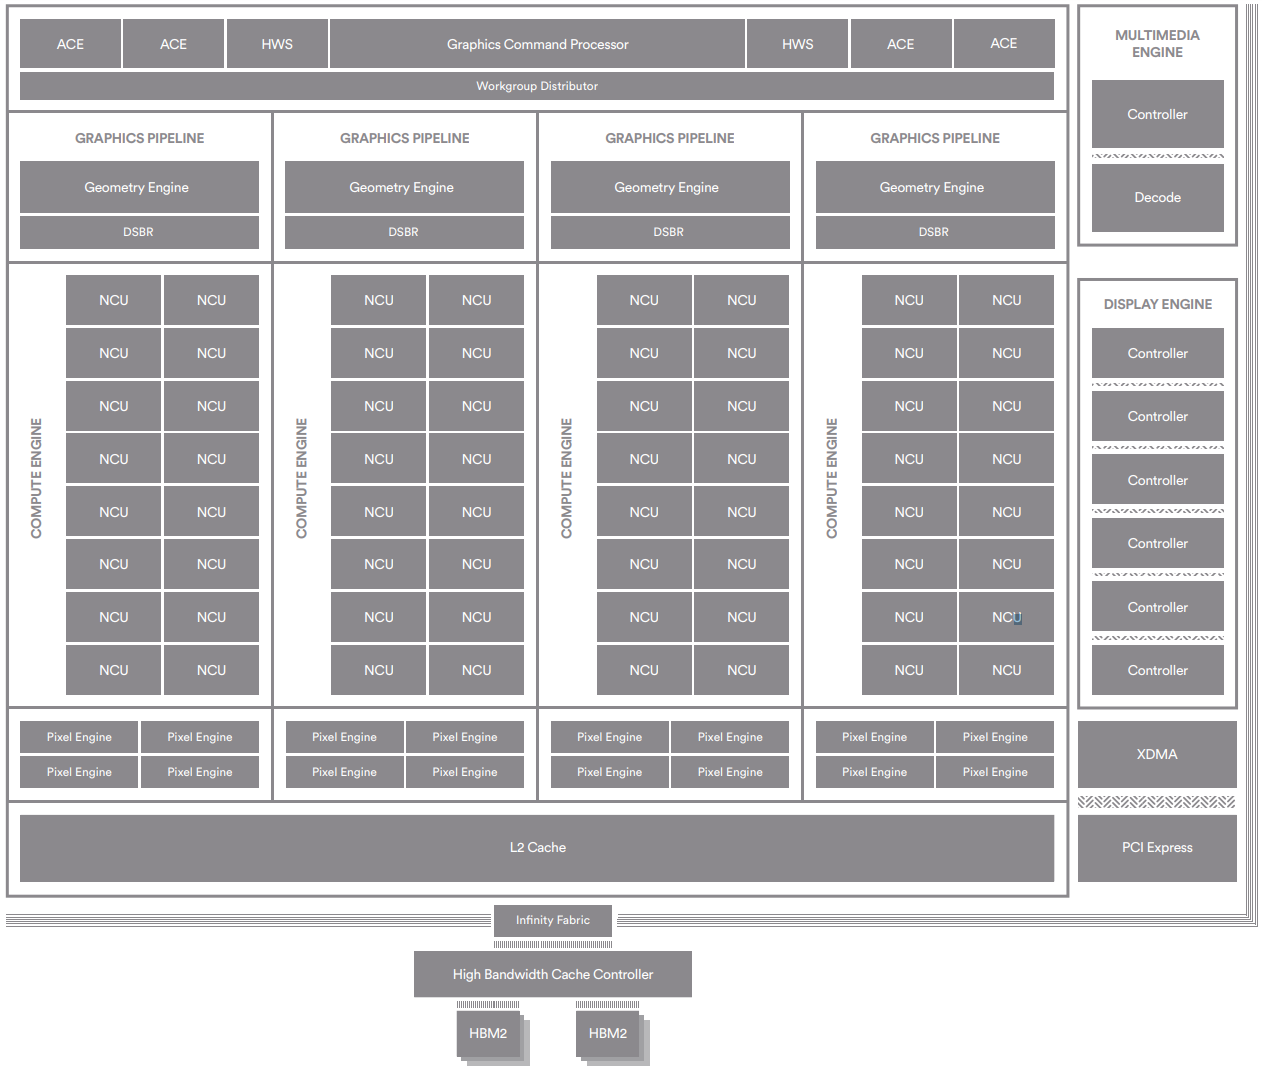
\includegraphics[width=0.7\linewidth]{Figures/StateArt/Vega10_microarchitecture.png}}
    \subfigure[NCU]{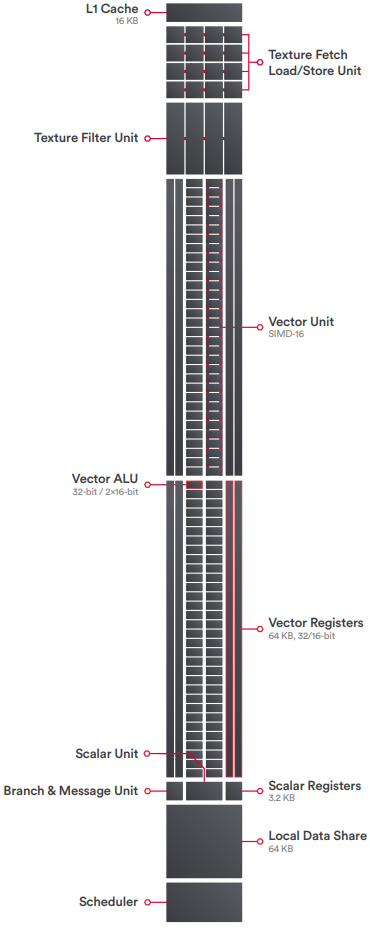
\includegraphics[width=0.29\linewidth]{Figures/StateArt/NCU.png}}
  \end{subfigmatrix}
  \caption{AMD's Graphics Core NExt logical Organization.}
  \label{fig:Vega10arch}
\end{figure}

In the fifth iteration of the GNC microarchitecture, AMD introduced a new memory hierarchy and support for High-Band Memory 2 (HBM2). In a conventional memory arrangement, the registers of each processing element pull data from a set of L1 caches, that, in turn, access the global L2 cache. Finally, the L2 cache system provides access to the GPU's video memory. This arrangement implies that the video memory has the entire working set of data and resources in order to provide high-bandwidth and low-latency access to data. However, in complex graphical scenes or while working GPGPU applications with large datasets, the total video memory may not be big enough to store all the data. In the Vega microarchitecture, by utilizing a  High-Bandwidth Cache Controller (HBCC), AMD made it possible to utilize the local video memory like a last-level cache. In this arrangement, when a missing piece of data, not currently stored in the local memory, is needed by the CUs, the GPU can pull just the necessary page memory from the host. In this setup, instead of the GPU stalling, while the entire missing resource is copied from the host throw the PCIe bus, it just needs to wait for the smaller page memory to be transferred, resulting in significantly decreased memory access times. The GPGPU applications take great advantage of this memory hierarchy since it enables the use of bigger datasets than the ones that could fit in video memory.

In the development of the work of this dissertation, a Radeon Vega Frontier Edition GPU is used. Table \ref{tab:gpusepcs} summarizes the most important specifications of the architecture of this device.

\begin{table}[!htb]
    \renewcommand{\arraystretch}{1.2} % more space between rows
    \centering
        \begin{tabular}{lc}
            \multicolumn{1}{c}{\textbf{}} & \multicolumn{1}{l}{\textbf{Radeon™ Vega Frontier Edition}} \\ \hline
            Base Architecture             & Vega GNC                                                   \\
            \#Compute Units               & 64                                                         \\
            \#Stream Processors           & 4096                                                       \\
            GPU Memory Size               & 16 GB                                                      \\
            Thermal Design Power          & 300 W                                                      \\ \hline
        \end{tabular}
    \caption{Characteristics of the used GPU device}
    \label{tab:gpusepcs}
\end{table}

\subsection{Radeon Open Compute platform}

The Radeon Open Compute (ROC) \cite{noauthor_radeonopencompute/rocm_2019} platform provides support for a set of frameworks and tools to allow developers to program and control the AMD GPUs. Figure \ref{fig:rocmplatform} shows the high-level organization of the platform. The platform includes a set of tools that allows developers to access ROC Kernel Driver data. In the following subsections, two of those tools, the ROCM-SMI \cite{noauthor_radeonopencompute/roc-smi_2019} and ROC-Profiler \cite{noauthor_rocm-developer-tools/rocprofiler_2019} tools, used on the development of this work, are described.

\begin{figure}[!htb]
  \centering
  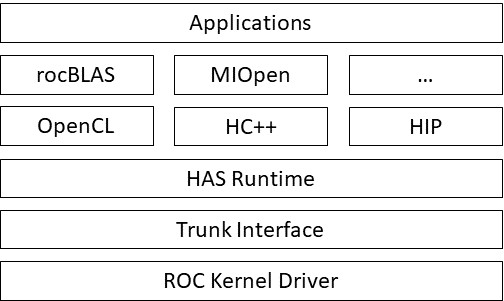
\includegraphics[width=0.4\textwidth]{Figures/StateArt/ROC_stack.jpg}
  \caption{Organization of the ROC platform.}
  \label{fig:rocmplatform}
\end{figure}

\subsubsection{ROCM-SMI}
The ROCm System Management Interface (ROC-SMI) \cite{noauthor_radeonopencompute/roc-smi_2019} is a user-friendly command-line application for manipulating the Radeon Open Compute Kernel (ROCK),  using it, is possible to know and control the state of the GPU device. The application uses sysfs files to query and manipulate the device kernel using the libsensors library \cite{noauthor_libsensors3:_nodate}.

From the set of query and control directives enabled by ROC-SMI, the following are of particular interest for the topic of this dissertation:

\begin{itemize}
\item \textbf{GPU utilization:} Retrieves the current utilization rates for the device's major subsystems, one value for the processing core and other for the main device memory. The rate is computed over a specific time interval set on the libsensors library. The processing core utilization reflects the percentage of time that the GPU core was being utilized to perform computations. In contrast, the main device memory utilization reflects the times on which the memory was being read or written.

\item \textbf{GPU power}: Retrieves the average power used by the device. Similarly to the utilization rate, the average power computed over the same time interval, during which a defined number of power samples are taken.

\item \textbf{Clock rate and voltage level:} Retrieves both the currently applied clock frequency and voltage level to the GPU core and the main device memory. It also displays two tables, the first, showing the eight pairs of clock frequency/voltage level of the GPU core and the second, showing four pairs of the same parameters related to the device memory. These two tables, correspondent to the 8 and 4 performance levels that the device kernel can apply to the GPU core and memory correspondingly.
\end{itemize}

The ROC-SMI interface also allows querying the device temperature, the current fan speed, and the selected performance level.

ROC-SMI also provides a mechanism to control and change device parameters such as:
\begin{itemize}
\item \textbf{Set clock rate and voltage level:} Set the clock frequency and the voltage level of any of the performance levels of both the GPU core and memory. 
\item \textbf{Set performance level:} Allows the user to select the desired performance level of the GPU core and device memory, disabling the driver automatic performance level management system.
\item \textbf{Reset clock rate and voltage level:} Resets the clock rates and voltage level to the default values.
\end{itemize}

Additionally, the interface allows the user to manually set the fan speed, necessary to guarantee the same temperature level for all executed tests

The versatility and total and independent control of the clock rate and voltage level of the device allowed by ROCM-SMI and the libsensors library was the defining factor for choosing an AMD GPU over the more popular options of NVIDIA. In the development of the work presented in this dissertation, an exploration of the voltage level is undertaken, and only the AMD platform allows for independent control over this variable.

\subsubsection{ROC-Profiler}

The Radeon Open Compute Profiler \cite{noauthor_rocm-developer-tools/rocprofiler_2019} is a profiling and tracing library for applications developed using any of the programming frameworks available on the ROC platform (OpenCL, HC++, HIP) \cite{sun_evaluating_2018}. The library gives access to the performance counters of AMD GPUs, allowing developers to configure the start, stop, read and reset of the physical registers on the microarchitecture that count the number of events (number of instructions per type, cache hits/miss) that the device is performing.

The instrumentation of applications with the API calls to ROC-Profiler allows for close monitoring of the type of operations being performed. The use of this tool can give valuable insights about the relation that the running code has with the utilized frequency and voltage and the produced result.


%%%%%%%%%%%%%%%%%%%%%%%%%%%%%%%%%%%%%%%%%%%%%%%%%%%%%%%%%%%%%%%%%%%%%%%%


\section{Dynamic Voltage and Frequency Scaling}
\label{section:dcvf}

The widespread use of GPUs in both supercomputers as on personal machines comes at the cost of a significant increase in the power consumption of the complete system. Whereas a typical modern CPU consumes about 50 to 100W, it is common to see GPUs rounding that value to 200 to 300W of power. With these figures, it is indispensable the use of energy efficiency techniques to try to reduce power consumption.

On any CMOS circuit, the total power consumed is decomposed into the dynamic and static parts. The dynamic power relates to the act of the transistors flipping their stages, and correspond to the power of charging and discharging the internal net capacitances. This value is proportional to the frequency that this change occurs. Equation \ref{eq:dynpower} represents the general form for dynamic power, where \textit{a} represents the utilization factor, \textit{C} the total capacitance of the circuit, \textit{V} the transistors supplied voltage and \textit{f} the operating frequency \cite{gonzalez_supply_1997}.

\begin{equation}
    P_{dynamic} = aCV^2f
    \label{eq:dynpower}
\end{equation}


On their turn, the static part of the power consumption is generated by $P_{leakage}$, $P_{short-circuit}$ and $P_{DC}$ \cite{mei_survey_2016}. The leakage power is independent of the transistors flip, and it represents the flow of electrons that exists between the transistors' source, drain, and gate. The short-circuit power comes from the instantaneous short-circuit connection between the supply voltage and the ground when the transistor flips. Finally, the Direct Current (DC) power corresponds to the power needed for powering the circuit. Equation \ref{eq:cmospower} represents the total power consumption sources.

\begin{equation}
    P_{total} = P_{dynamic} + P_{leakage} + P_{short-circuit} + P_{DC}
    \label{eq:cmospower}
\end{equation}

The dynamic power dominates the total power consumption of a circuit, however, with the reduction of the manufacturing size of the transistor seen nowadays, the static power is also contributing heavily \cite{s._hong_modeling_2012} \cite{hong_integrated_2010}. As a common reference, due to the higher height of the dynamic power on the total power consumption, the power used by a circuit changes linearly with the clock frequency and quadratically with the supplied voltage.


By intelligently controlling the clock frequency, the necessary voltage for stable operation of the circuit can also be reduced, leading to power savings. However, the reduction of the operating frequency harms the pic performance of the circuit, so a careful scaling of voltage/frequency needs to be done in run-time. The "on the fly" control of these parameters is called Dynamic Voltage and Frequency Scaling (DVFS). This power management technique allows for an energy efficiency improvement by matching the GPU utilization to the voltage and frequency apply to it.

In general, modern GPU boards have independent control over two pairs of frequency and voltage. Each pair or domain acts on a distinct part of the GPU, intending to maximize the performance or reduce the power consumption. The first domain concerns the GPU core, acting on all CUs, the cache, and the interconnection fabric. The second affects the DRAM chips that compose the video memory. 

The clock frequency is an independent control variable, and its change is reflected directly on the performed achieved by the GPU. An increase in the clock frequency of the core results in an improvement of the CU execution speed, while the same change in the memory frequency will increase the DRAM I/O throughput \cite{mei_survey_2016}. The voltage level of each domain is dependent on the clock frequency and is computed based on tests performed by the manufacturer that ensure the correct operation of the circuit, independently of the workload.

Both AMD and NVIDIA have on their products the concept of performance levels, that is, a set of pairs of frequency and voltage that can be applied to the many components of the GPU. These vary from low power and performance levels to high performance and high power ones. The idea of having multiple performance levels is to be able to always be at the best point of operation.  In the case of AMD, the GPU core has eight possible pairs, table \ref{tab:gpucorelevels} shows the reference values of frequency and voltage for each of the core performance levels, while the GPU memory has only four, table \ref{tab:gpumemlevels}. Through the use of software like ROC-SMI \cite{noauthor_radeonopencompute/roc-smi_2019} the user can input the desired combination of values for each level, allowing for an almost continuously selection of values for the frequency and voltage within the specifications range. For example, on the Vega 10 Frontier Edition used on the experimental work of this thesis, the GPU core frequency can be set between 852 and 1980 MHz and the GPU memory frequency between 167 and 1500 MHz. In turn, the voltage can be set between the 800 and 1250 mV. As stated before, the primary benefit of AMD over NVIDIA's solution is that this manufacturer allows for the override of the automatic computation of the GPU voltage. This difference is of significant importance since it allows finer control of the DVFS values and a more interesting possibility of exploration of the voltage level.

\begin{table}[!htb]
\renewcommand{\arraystretch}{1.2} % more space between rows
\centering
\begin{tabular}{ccc}
\textbf{Level} & \textbf{Frequency {[}MHz{]}} & \textbf{Voltage {[}mV{]}} \\ \hline
0              & 852                          & 800                       \\
1              & 991                          & 900                       \\
2              & 1138                         & 950                       \\
3              & 1269                         & 1000                      \\
4              & 1348                         & 1050                      \\
5              & 1440                         & 1100                      \\
6              & 1528                         & 1150                      \\
7              & 1600                         & 1200                      \\ \hline
\end{tabular}
\caption{GPU Core Levels of Frequency and Voltage of AMD Vega 10 Frontier Edition}
\label{tab:gpucorelevels}
\end{table}

\begin{table}[!htb]
\renewcommand{\arraystretch}{1.2} % more space between rows
\centering
\begin{tabular}{ccc}
\textbf{Level} & \textbf{Frequency {[}MHz{]}} & \textbf{Voltage {[}mV{]}} \\ \hline
0              & 167                          & 800                       \\
1              & 500                          & 900                       \\
2              & 800                          & 950                       \\
3              & 945                          & 1000                      \\ \hline
\end{tabular}
\caption{GPU Memory Levels of Frequency and Voltage of AMD Vega 10 Frontier Edition}
\label{tab:gpumemlevels}
\end{table}

\subsection{Control Mechanism}

The correct choice of the most appropriate performance level for each of the GPU clock domains is one of the topics of more research from both the manufactures and researchers. The correct design of the DVFS controller has a significant impact on the energy efficiency of the GPU.

The first implementations of GPU DVFS controllers took direct inspiration from the CPU DVFS. These used strategies like scaling up the processor frequency, race-to-idle \cite{hoffmann_racing_2013}, when a task is launched in the pursuit of finishing it as fast as possible and return to an idle state. However, "racing", as described in \cite{kim_racing_2015}, that prof to increase the energy efficiency of CPUs, does not always result in the same outcome for GPUs \cite{kim_racing_2015}.

In general, the challenges of creating a better GPU DVFS relates to three factors. The GPU power management is very limited, the lack of accurate quantitative GPU DVFS performance and power estimation tools, and the fact that the GPU architecture design is still evolving rapidly, which makes the strategies applied to one architecture design have different outcomes on the next iteration of it \cite{mei_survey_2016}.

%%GPGPU-Perf: efficient, interval-based DVFS algorithm for mobile GPGPU applications
%Many DVFS algorithms to properly predict applications’ workloads have been proposed originally on the CPU side. These can be largely classified into three categories: interval-based, inter-tasks, and intra-tasks algorithms [3]. Interval-based algorithms periodically measure how much busy a device is during the given time (i.e. utilization), and setthenextvoltageandfrequencybasedonthecurrentmeasurementofutilization.Theutilization,Ui,canbeformulated by Eq. 2 when Ti is a time interval at time frame i, and the GPU spends time, wi, for working.


The control mechanism of the GPU DVFS used nowadays by both AMD and NVIDIA is schematized on figure \ref{fig:DVFSmechanism}. The most recent AMD GPU DVFS mechanism is called Adaptive Frequency and Voltage Scaling (AVFS) \cite{amd_polaris_nodate}. AFVS takes into account the voltage levels across the different parts of the GPU, the die temperature, the frequency and, the total power consumption. The objective of the controller is to maintain the total power consumption within the required power and temperature envelope, this is, for a given power target, when launching a new task, the GPU tries to achieve the highest possible frequency (highest performance level). For that, it adjusts the voltage level to the one required to correct functioning. With the use of the highest performance level, power, and temperature increases, when one of these parameters achieves the limit, the GPU decreases to a lower performance level to maintain itself within the power and temperature target. 

\begin{figure}[!htb]
  \centering
  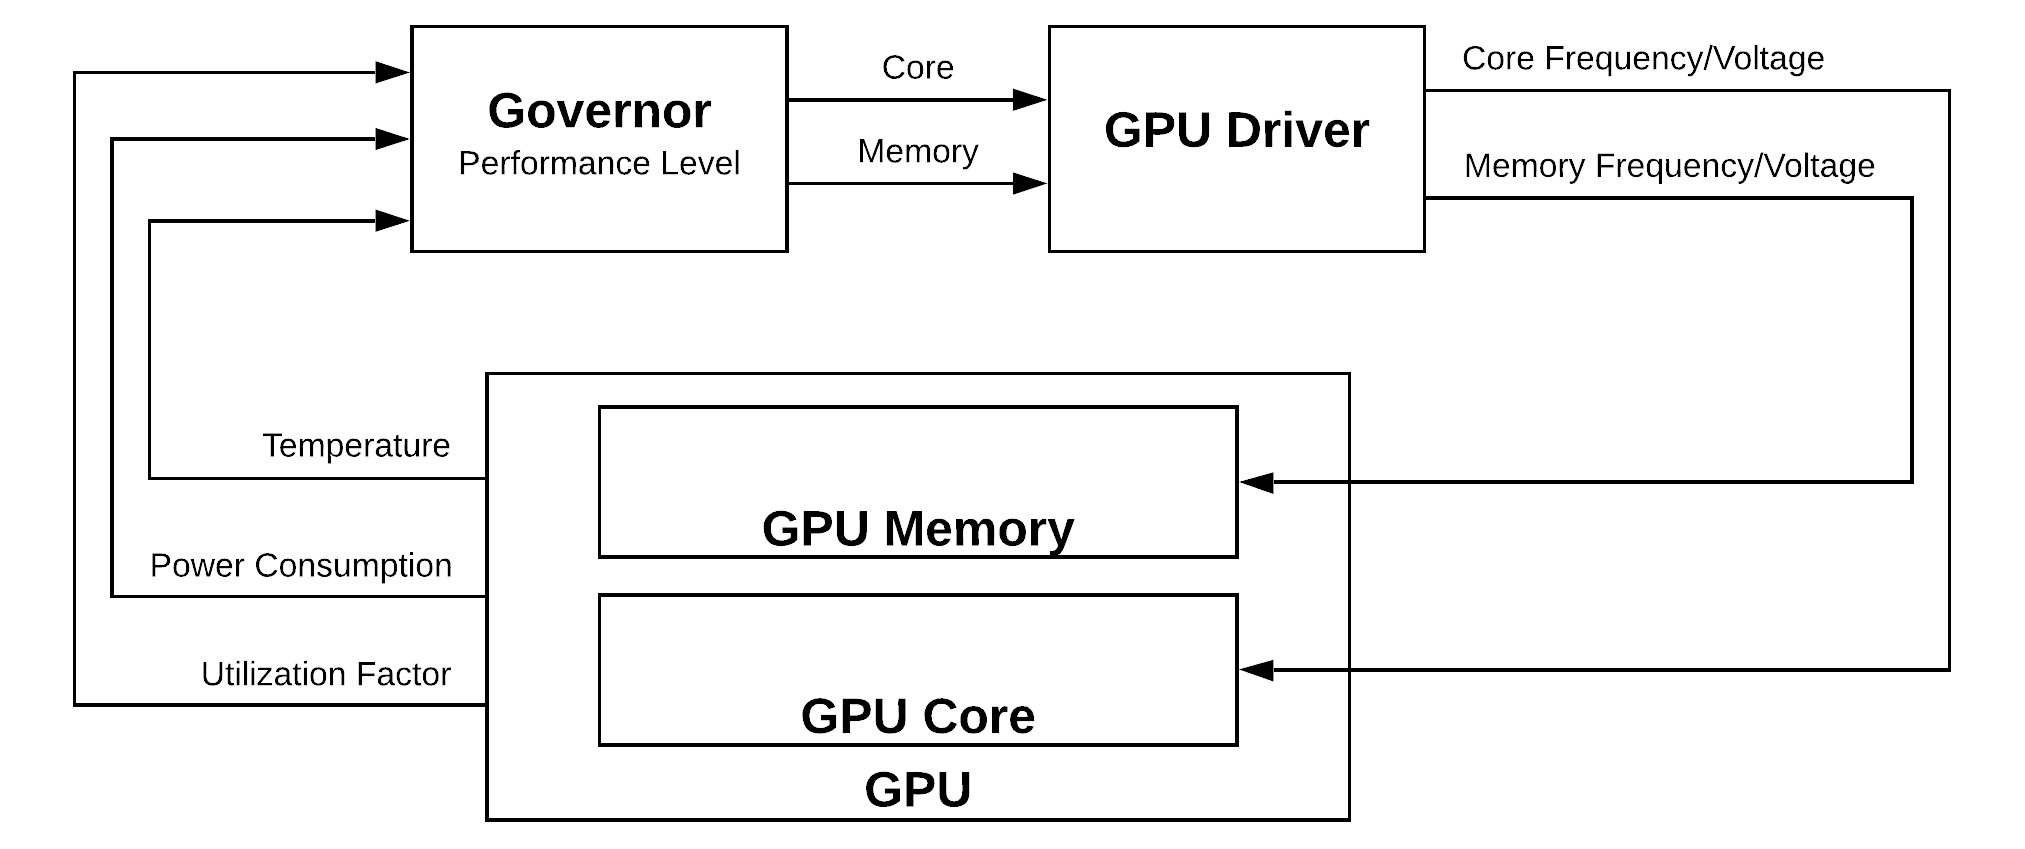
\includegraphics[width=0.75\textwidth]{Figures/StateArt/DVFS.png}
  \caption[Controller]{DVFS control mechanism.}
  \label{fig:DVFSmechanism}
\end{figure}

The major drawback of the current implementation of GPU DVFS is not taking into account the type of task that the GPU is solving. The dominant control mechanism still considers the GPU as a block box and controls its DVFS settings, only looking to outside parameters. The black box approach is enabling significant improvements in the energy efficiency of the device; however, it lacks the optimization of the frequency/voltage to the type of workload. For instance, a given application can be compute-bound or memory-bound, depending on if the time that it takes to performed is limited by the processor performance or the memory throughput. A compute bounded application can be limited by different components of the processor architecture, depending on the type of data (integer or floats) and the intended precision (size of the operands). If one compares the computation with the same type of operands but with different precision, for instance, 16 vs. 32 bits, even though the GPU is using the same arithmetic unit, the critical path for 32 bits operands is of increased length. That is, the maximum delay between the input and output for operations increases with the precision of the operands. Though, since the same clock frequency is used in both cases, the voltage level needs to be set at a level that ensures that the transistors flip at fast enough rate for the case with the highest precision. Considering that the manufacturers do not tune their devices to the minimum voltage level, to accommodate for manufacturing imprecisions and to leave a safe guard-band, the operating voltage of the circuits can be significantly reduced, leading to significant power savings. 

Overall, the minimum operating voltage of each performance level is set at a level high enough, that ensures the correct functioning of the processor, independently of the computations being performed. Nevertheless, it is possible to fine-tune the voltage and frequency if the type of task being executed is known.

\subsection{GPU DVFS Characterization and Effects}

Being the GPU such a widely used computation platform, in order to improve their performance and energy efficiency, it is of significant matter the characterization and analysis of the DVFS effects, mainly on understanding the impact of the different parameters on different workloads scenarios. A complete GPU DVFS characterization is explored in the literature using two methodologies. The first is experimental studies, where researchers use real GPUs to perform voltage and frequency scaling. Due to past dominance of NVIDIA over AMD \cite{noauthor_jon_nodate} \cite{mujtaba_amd_2019} and the fact that this manufacturer only offers limited support for independent voltage scaling tools, the majority of the work act solely on frequency scaling. The second approach uses simulators, like GPUWattch \cite{noauthor_gpu_nodate} or GPGPU-Sim \cite{noauthor_gpgpu-sim/gpgpu-sim_distribution_2019,},  to simulate various scaling approaches like GPU core number scaling and per-core DVFS \cite{mei_survey_2016}. The benefit of using simulators over real hardware comes on the increased flexibility allowed by the previous, permitting for the experimentation of scenarios not supported by the frequency/voltage scaling tools provided by the manufacturers. In both methodologies, the studies act on the impact on performance and energy consumption/efficiency.

%https://www.researchgate.net/publication/261725696_A_Survey_of_Methods_For_Analyzing_and_Improving_GPU_Energy_Efficiency

% Falar que se pode aproveitar TI applications para explorar os limites minimos


%ASurveyandMeasurementStudyofGPUDVFSonEnergyConservation
%In our previous work [47], we introduce the methodology to scale the core and memory voltage/frequency of the Fermi GPU, with the help of a series of third-party software tools. For the Maxwell platform, we use the NVIDIA Inspector [58] to scale the core/memory frequency. In addition, we disableGPUBoosttofixtheGPUcore/memoryfrequencyat the selected level. The NVIDIA Inspector reports the power data every second

%Aggressive Voltage and Temperature Control for Power Saving in Mobile Application Processors
%Study the effects of a temperature aware DVFS on mobile devices to relate with the TEMPERATURE INVERSION PHENOMENON 
%We demonstrated that the T-DVS can achieve power saving with aggressive voltage control by capitalizing on the relationship between operating voltage and temperature. We expect the T-DVS to set a milestone in active voltage control for power management in mobile devices. The effectiveness of the T-DVS was achieved solely by using software approaches and employing existing hardware features. 

\subsubsection{Experimental}
\subsubsection{Simulation}
%%%%%%%% EXPERIMENTAL

%ASurveyandMeasurementStudyofGPUDVFSonEnergyConservation
%Jiao et al. scaled the core frequency and the memory frequency of a NVIDIA Tesla GTX280 GPU with three typical applications: the compute-intensive dense matrix multiply, thememory-intensivedensematrixtranspose,andthehybrid fast Fourier transform (FFT) [31]. The three applications showed different performance and energy efficiency curves with the same core-memory frequency settings: the dense matrix multiply was insensitive to memory frequency scaling, FFT benefited from low core frequency and high memory frequency, while dense matrix transpose needed both high core and memory frequency. They also found that the energy efficiency was largely determined by the instructions per cycle (IPC) and the ratio of the amount of global memory transactions over the amount of computation transactions. 
%Ge et al. applied fine-grained GPU core frequency and coarse-grained GPU memory frequency on a Kepler K20c GPU, and compared its effect to the CPU frequency scaling [19]. They found that for dense matrix multiply, both the GPU power and the GPU performance were linear to the GPU core frequency, and the GPU energy consumption was insensitive to frequency scaling. For their three tested applications, the highest GPU frequency always resulted in best energy efficiency, differing from the CPU DVFS. 
%In our previous work, we scaled the core voltage, the core frequency and the memory frequency of the Fermi GTX560Ti GPU, with a set of 37 GPU applications [47]. We found that the effect of GPU DVFS depends on the application characteristics. The optimal setting to consume the least energy was a combination of appropriate GPU memory frequency and core voltage/frequency. We observed an average of 20% reduction of energy consumption with only 4% of performance loss. 
%Abe et al. combined the GPU core frequency, the GPU memory frequency and the CPU core frequency scaling together, on the NVIDIA Fermi GTX480 GPU [3]. They performed the frequency scaling with dense matrix multiply of various matrix sizes. They could save as much as 28% of the system energy with a small matrix size, low GPU memory frequency and high GPU core frequency. They then extensively scaled the GPU core and memory frequency of 4 GPU products, including the Tesla GTX285, Fermi GTX460/GTX480, and Kepler GTX680, with 33 popular applications [2]. They set both of the core and memory frequency to low, medium and high values, and searched for theoptimalcore-memoryfrequencycombinationthatoffered the best power efficiency. Surprisingly, they found that, for the Kepler GTX680, the default frequency configuration was never optimal, while the opposite for the Tesla GTX285. They could reduce as much as 75% of system energy within 30% of performance loss, for a compute-intensive workload on the Kepler GPU. Their results suggested that DVFS was even more appealing for recent GPUs.
%YouandChungdesignedaperformance-guaranteedDVFS algorithm for the Mali-400MP GPU on a SoC platform [75]. They found that the GPU utilization ratio was not tightly correlated to the GPU performance, and the ondemand DVFS provided by the SoC system was inadequate by wasting a certain amount of power. 
%Jiao et al. studied the GPU core and memory frequency scaling for two concurrent kernels on the Kepler GT640 GPU [30]. They took a set of kernels from the CUDA SDK andRodiniabenchmarkandmeasuredtheirenergyefficiency (GFlops/Watt) with different core-memory frequency settings. They demonstrated that the concurrent kernel execution in combination with GPU DVFS can improve energyefficiency by up to 34.5%. 

%MAXWELL: The authors of the paper scale the frequency and gather the energy consumption of a set of Rodnia benchmars. They show that some benchs benefict (energy efficiency) from underclocking and others from overclocking. Some apps increase the energy consumption linearly, others are insensitive to frequency, others present an optimal setting. The authors show that underclocking the memory results in great energy consumption increase (due to longer execution time). They conclude that the default setting is the best one. For the few kernels that reduce energy consumption with memory overclock is due to the reduce execution time outshadows the energy increase on the memory
%FERMI: Authors scale down both core clock and voltage, achieve great energy reduction. Best energy at lowest voltage/frequency. Dont find a relation between memory DVFS and energy/performance.
% Appropriate core frequency setting is effective for energy saving. Both platforms expose the “pacing [34]” feature. The relationship between the performance and the GPU core frequency is very complex and a simple linear model is inadequate; 2) In terms of memory frequency scaling, the early platform exposes the “pacing” feature, while the modern platform exposes the “racing [34]” feature. The performance is highly linear to the GPU memory frequency on our Maxwell platform.
%Highly platform /architecture dependent


% A Survey of Methods For Analyzing and Improving GPU Energy Efficiency
%Jiao et al. [2010] study the the performance and power consumption of GPU for three computationally diverse applications for varying processor and memory frequencies. Specifically, they study dense matrix multiplication (compute-intensive), dense matrix transpose (memory-intensive), and fast Fourier transform (hybrid). They have observed that the power consumption of GPUs is primarily dependent on the ratio of global memory transactions to computation instructions and the rate of issuing instructions. These two metrics decide whether an application is memory-intensive or computation-intensive, respectively. Based on these characteristics, the frequency of GPU cores and memory is adjusted to save energy

%Aggressive Voltage and Temperature Control for Power Saving in Mobile Application Processors
% Leng et al. [6] endeavored to reduce the voltage guardband that is incorporated in conventional GPU operation. The authors pointed out that the guardband for voltage noises stems from various program behaviors and optimized the guardband with offthe-shelf GPUs used in desktops
%A few recent works centered on voltage optimization. Bacha et al. [4], [5] achieved dynamic voltage reduction using on-chip error correction code-based voltage speculation. A benchmark test with a specific firmware demonstrated that approximately 20 percent power conservation is possible with aggressive voltage reduction over Intel’s Itanium processor
% near-threshold voltage (NTV) technology emphasizes the importance of reduced operating voltage. Kaul et al. [29] introduced the concept of NTV and demonstrated that maximum energy efficiency can be achieved using this technology. Intel demonstrated the effectiveness of an NTV Pentium processor [30] that runs on very low power. Voltage down using software techniques facilitates the NTV scheme. 


%%%%%%% SIMULATION

%ASurveyandMeasurementStudyofGPUDVFSonEnergyConservation
%In [37], Lee et al. simulated the GPU DVFS as well as the core number scaling in GPGPUSim, based on the 32nm prediction technology model [78], with the objective to improve the throughput. Their scaling scheme can provide an average of 20% higher throughput than the baseline GPU. 

%Leng et al. developed GPUWattch, which could simulate the cycle-level GPU core voltage/frequency scaling, based on the Fermi GTX480 GPU [38]. They configured the various GPU voltage/frequency settings according to the 45nm prediction technology model [78], [10], and simulated both slow off-chip and prompt on-chip DVFS. They gained an average of 13.2% energy saving with off-chip DVFS and 14.4% energy saving with on-chip DVFS, both within 3% performance loss. For either scaling scheme, they found that the memory-bounded kernels benefited a lot but the purely compute-bounded kernels did not take much advantage of the DVFS. 

%Sethia et al. designed a dynamic runtime GPU core number, core and memory frequency scaling system, to either conserve the energy or improve the performance [64]. They categorized the GPU applications into 3 types: computeintensive, memory-intensive, and cache sensitive, according to GPUWattch characterizations. For each application category and scaling objective, they designed different scaling strategies. Their system reduced 15% energy in the energysaving mode. Sen et al. applied the fine-grained per-core DVFS in GPUWattch, in view of the diverse execution time and workload of different GPU cores [63]. They found the percore DVFS had good potential to save more power than the overall DVFS. Motivated by the fact that scaling down the core voltage was vital to conserve energy, Gopireddy et al. designed a new architecture that enabled a lower operating voltage in the energy-efficiency mode other than the normal voltage in the high-performance mode [23]. Their simulation results showed that the new hardware could reduce as much as 48% of energy consumption, compared to the conventional hardware with normal DVFS. In summary, GPU DVFS is proved to be effective in energy conservation for a variety of applications, but the impact on different applications are very diverse. Researchers need to design specific scaling algorithm based on the application characteristics. 

%Core-level DVFS for Spatial Multitasking GPUs 
%It is difficult to analyse DVFS when in spatial multitasking, and determine the optimal DVFS. Created GPU simulatoor, operates DVFS at the SM level
% They used Rodinia suite[6], Parboil suite[5] and Polybench suite [7]. benchs and combine (Com + Com), (Mem + Mem), and (Mem + Com)  apps , measure IPC for perforamce metric becasuse the clock period of one cycle varies when the frequency changes. 
%Com+ COM - Executing two computeintensive kernels with a 20 % increase in the SM frequency (in the case of H+H) resulted in a 20.4% increase in the performance compared with the baseline (N+N). Conversely, when the SM frequency was reduced by 20% (L + L), the performance was reduced by 19.3% compared with the baseline. performance has been changed linearly by the frequency of the SM where the kernel is running
%2) Mem+Mem Cases -  the performance did not change significantly depending on the SM frequency
%3) Mem+Com Cases : By increasing the frequency of all SMs by 20% (H + H), the performance of the memory-intensive kernels increased only by 3.7% compared with the baseline but the performance of the computeintensive kernel increased by 11.5%. For the (L + L) case, the performance of the memory-intensive kernel and the computeintensive kernel decreased by 5.8% and 17.3%, respectively. The performance of the (H + N) case was similar to the baseline. The performance of the (H + L) case was similar to that of the (N + L) case. In the (Mem + Com) configuration, the performance of compute-intensive kernel in the (N + H) case was the best, which improved the performance by 17.4% compared with the baseline. This performance gain is higher than that of the (H + H) case and power consumption is also expected to be less.  
 %Over and underclock of 1/4 - draw back is the added hardware




\subsection{DVFS Optimization}

Relevant work is being done on finding improvements to the current GPU DVFS system. The investigation divides on the DVFS characterization, on architectural changes to DVFS, and, on the creation of novel control mechanisms. GPU DVFS characterization works explore how does the performance and energy efficiency relate to DVFS settings, using different kinds of workloads. The study on architectural changes to DVFS investigates how does the creation of more clock/voltage domains is beneficial for the energy efficiency of the device. The last category searches how can more complex, aware DVFS systems, better control the voltage and frequency depending on the workload type.



\subsubsection{Architectural changes}

% A Survey of Methods For Analyzing and Improving GPU Energy Efficiency
%Nam et al. [2007] propose a low-power GPU for hand-held devices. The proposed GPU uses logarithmic arithmetic to optimize area and power consumption. The use of logarithmicarithmetic leads to some computation error, however, due to the small screen of the handheld devices, the error can be tolerated. They divide the chip into three power domains, viz. vertex shader, rendering engine and RISC processor, and DVFS is individually applied to each of the three domains. The power management unit decides the supply voltage and frequency of each domain based on its workload for saving power while maintaining the desired performance level




\subsubsection{Novel DVFS mechanisms}
%Clock splitting technique
%grande margem para fazer tudo, nao optimizado


%ASurveyandMeasurementStudyofGPUDVFSonEnergyConservation
%Falam que ha espaço para DVFS aware



%GPGPU-Perf: efficient, interval-based DVFS algorithm for mobile GPGPU applications
% GPUs can be used to two types of workloads, graphics and GPGPU. In graphics, there's a objective of 30/60 fps to be met, when over performance is available, we can decrease the F and V. However, in GPGPU, GPU should process them as fast as possible. They create a new GPGPU-Perf algorithm that adjusts the DVFS params (threshold and interval) which results performance over energy increases by 1.44 times with no influences on graphic tasks and any modifications of GPGPU algorithms.
% They expand OpenCL to include a DVFS programming interface. If only a single set of thresholds is available regardless of the presence of graphic or GPGPU tasks, it makes sense thatgraphicapplicationshaveahigherprioritythanGPGPU applicationstodeterminethethresholds, HU and HD,mainly because the number of existing graphic applications in the fieldsismuchhigherthanthatofGPGPUapplications.
% weighted thresholding based on working times, adaptive interval adjustment based on utilization changes and multi-level frequency adjustment based on previous utilization. he performance 2.04 times with energy consumption 1.51 times via intelligent frequency controls.

 



%%%%%%%%%%%%%%%%%%%%%%%%%%%%%%%%%%%%%%%%%%%%%%%%%%%%%%%%%%%%%%%%%%%%%%%%
\section{Models}

%DVFS-aware application classification to improve GPGPUs energy efficiency
% novel DVFS-aware performance and power classification models are herein proposed that correlate application characteristics and GPU architecture features. In particular, by analysing the utilization of graphics and memory components at a single voltage and frequency levels, the proposed classification methodologies are able to pre dict the impact of DVFS on GPGPU applications execution time and power and energy consumption. 
%Authors explain how a compute baunded app can become mem and the reverse depending on the mem frequency. A simple binary classifier doesnt do the work
\subsection{Power Modeling}


%ASurveyandMeasurementStudyofGPUDVFSonEnergyConservation
%In this section, we survey the runtime GPU power modeling work. We classify the studies into either empirical or statistical, where the former one relies on the binary code analysis andthe latter one relies on the program performance counters. The empirical method is a bottom-up approach and requires break-up of GPU micro-architectures, while the statistical method treats the GPU hardware as a black box and seeks statistical relationships between the GPU power and the runtime performance counters. 
\label{section:powermodels}
\subsubsection{Empirical Methods}
\subsubsection{Statistical Methods}

\subsection{Performance Modeling}
%ASurveyandMeasurementStudyofGPUDVFSonEnergyConservation
%In this section, we introduce the GPU performance modeling studies, where a number of them consider the GPU frequency scaling. We classify them into two categories: pipeline analysis and statistical methods. The pipeline analysis is a bottom-up empirical method which requires the knowledge of GPU execution principles, while the statistical methods purely rely on the GPU performance counters. 
\label{section:powermodels}
\subsubsection{Pipeline Analysis}
\subsubsection{Statistical Methods}
Performance Counters

\section{Related Work}

\section{Summary}


For the early processing units, the dynamic power accounts for the majority of power consumption, but nowadays the static power is also contributing considerably